\documentclass{article}
\usepackage{listings}
\usepackage{graphicx}
\usepackage{adjustbox}

\begin{document}
\begin{enumerate}
\item \begin{minipage}[t]{\linewidth}
          \raggedright
          \adjustbox{valign=t}{%
            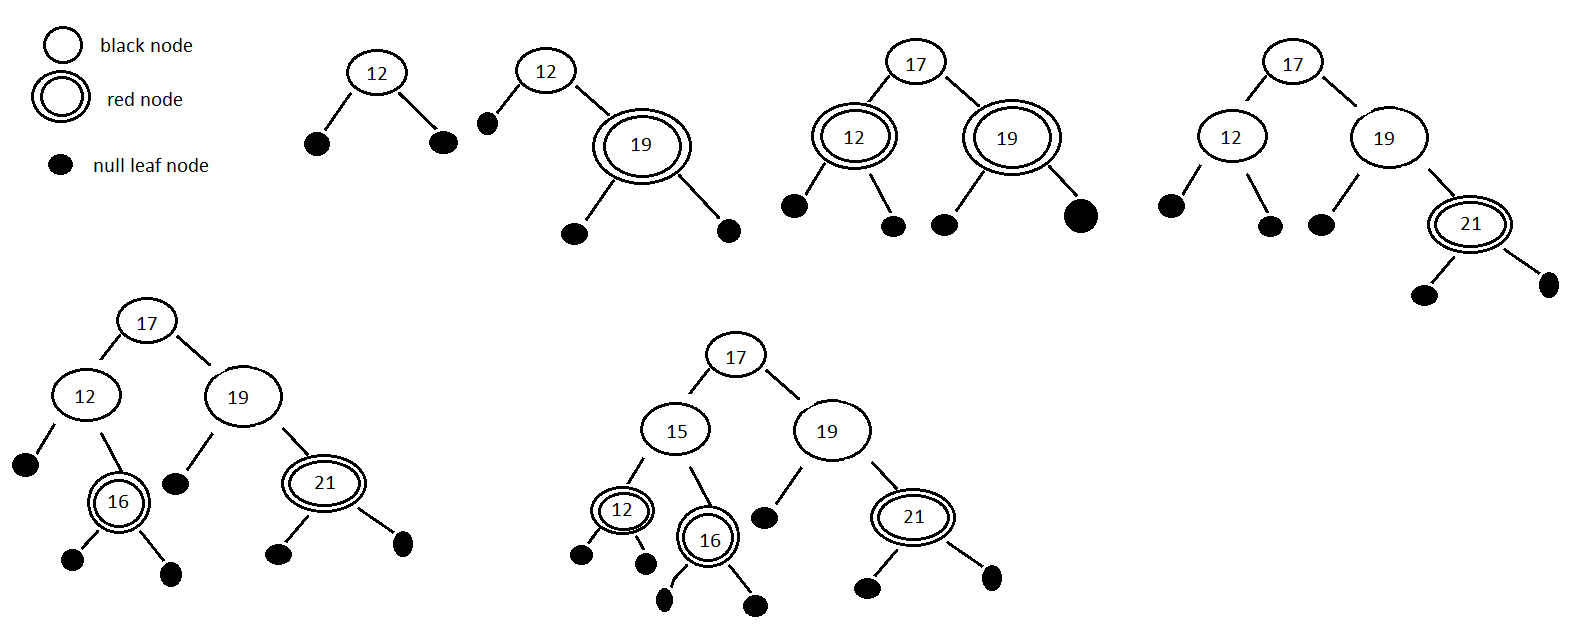
\includegraphics[width=.8\linewidth]{Problem1.png}%
         	 }
	\end{minipage}
\item \begin{minipage}[t]{\linewidth}
          \raggedright
          \adjustbox{valign=t}{%
            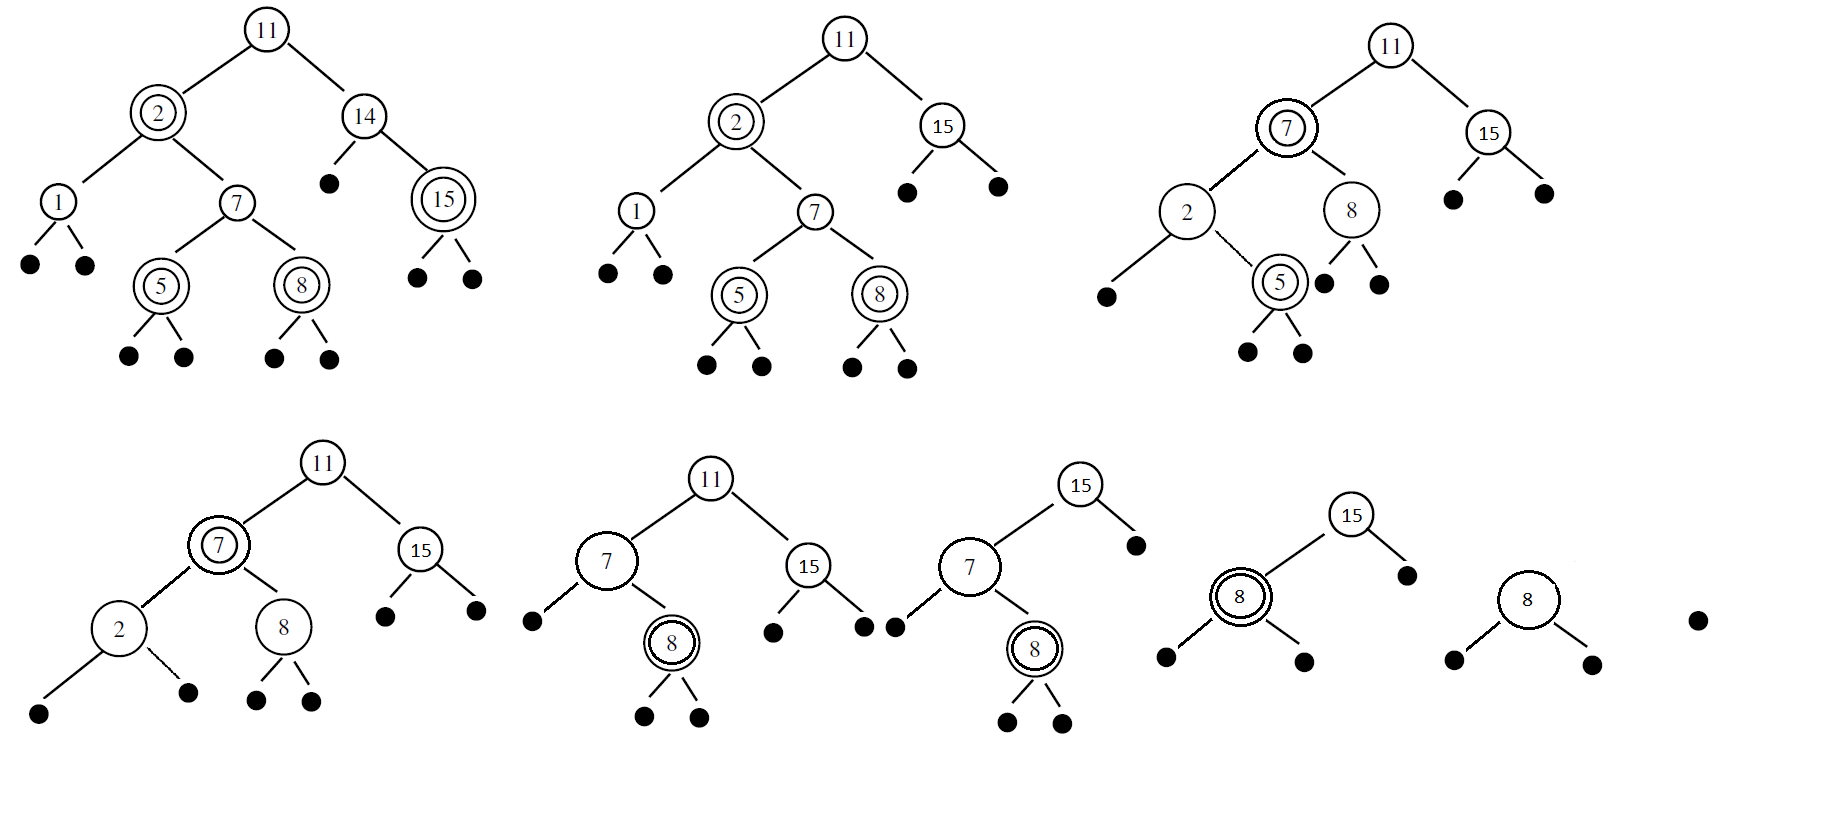
\includegraphics[width=.8\linewidth]{Problem2.png}%
         	 }
	\end{minipage}
\item\begin{minipage}[t]{\linewidth}
          \raggedright
          \adjustbox{valign=t}{%
            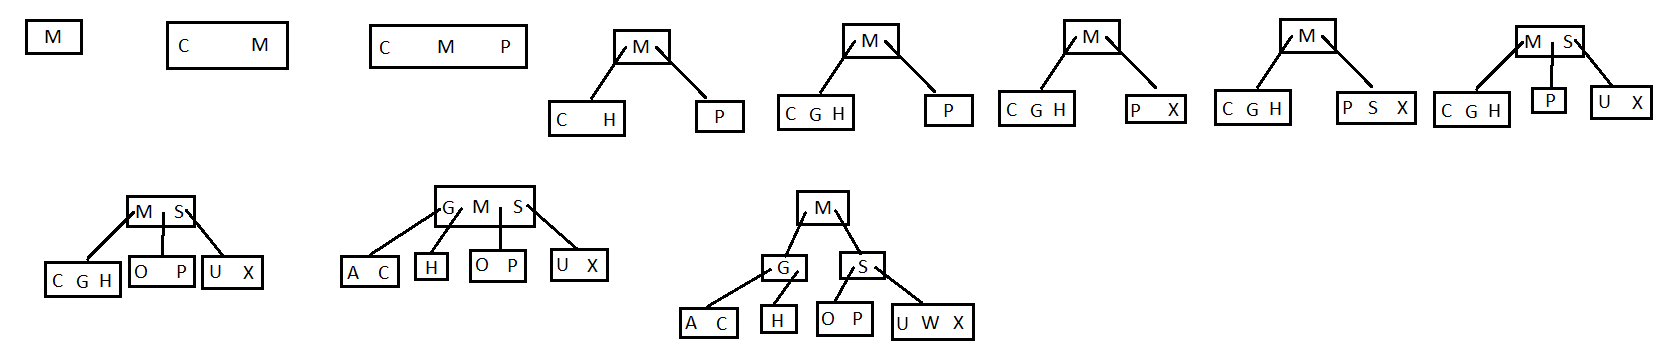
\includegraphics[width=.8\linewidth]{Problem3.png}%
         	 }
	\end{minipage}
\item \begin{minipage}[t]{\linewidth}
          \raggedright
          \adjustbox{valign=t}{%
            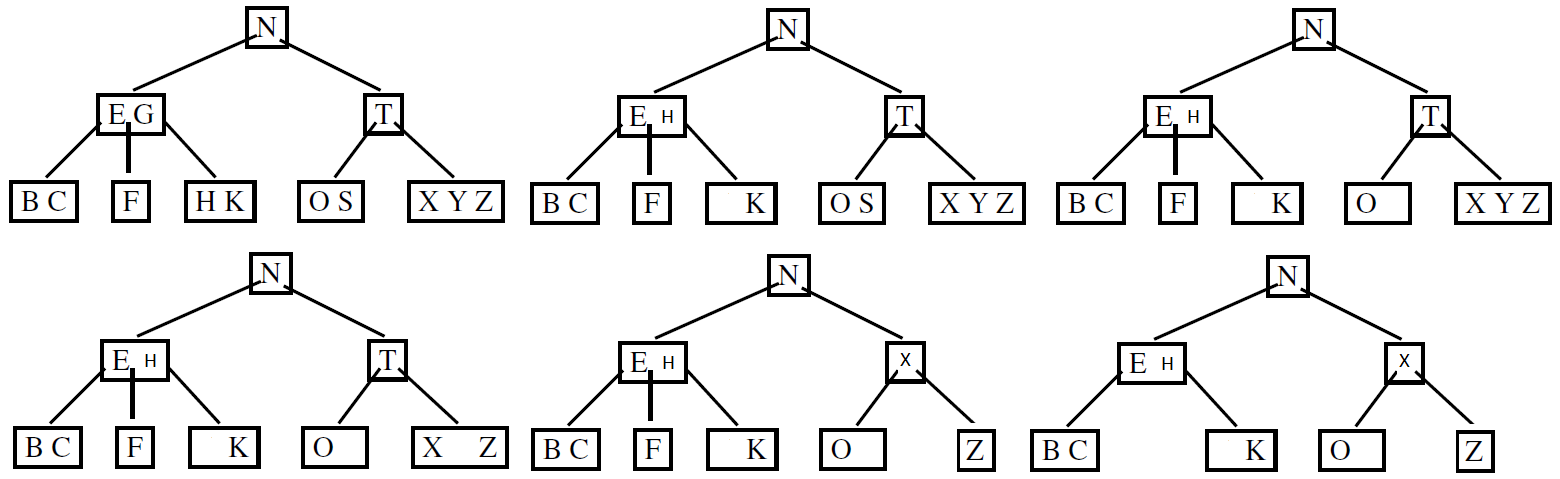
\includegraphics[width=.8\linewidth]{Problem4.png}%
         	 }
	\end{minipage}
\item An idea for finding the max value would be to traverse the nodes furthest to the right until the right-most leaf node is reached and then returning a reference to that node as well as
	the key in the right-most position inside the node.\\
	An idea for finding the predecessor of a given node would be to use the previous max function with the input being a reference to the given node/key index's pointer on the left
	 side while checking all edge and special cases. \\\\\\\\\\\\
	\begin{lstlisting}
B_tree_max(root){
	Node n1 = root;
	Node n2;
	while(n1!=null){
		n2=n1;
		n1=n1.pointers[pointers.length-1];
	}
	return n2, n2.keys[keys.length-1];
}

B_tree_predecessor(node, i){
	if(node.pointers[i-1]!=null){
		return B_tree_max(node.pointers[i-1]);
	}
	Node y = node.parent;
	key  k = node.keys[i];
	int index = i;
        while (y != null) {
	for(int i=0; i<y.keys.length-1; i++;){
		if(y.keys[i]>k){
			if(i==0){break;}else{//breaks while loop
			index=i-1;}
		}
	}
            node = y;
            y = y.parent;

        }
        return y, index;
}
	\end{lstlisting}
\item An idea would be to create a B-Tree and load the data into nodes with each node containing at most 1 page of data (2t-1=number of elements in a page) and then utilize the in-order
	traversal funtion to display the data in each node in a sorted order. Because of the definition of a B-Tree, the nodes will still be visited in order using that function, however, one
	would have to put the recursive calls and print statement in a loop in order to reach all of the nodes in the pointer array and keys in the keys array.
\end{enumerate}
\end{document}
